\begin{figure}[H]
	\centering
	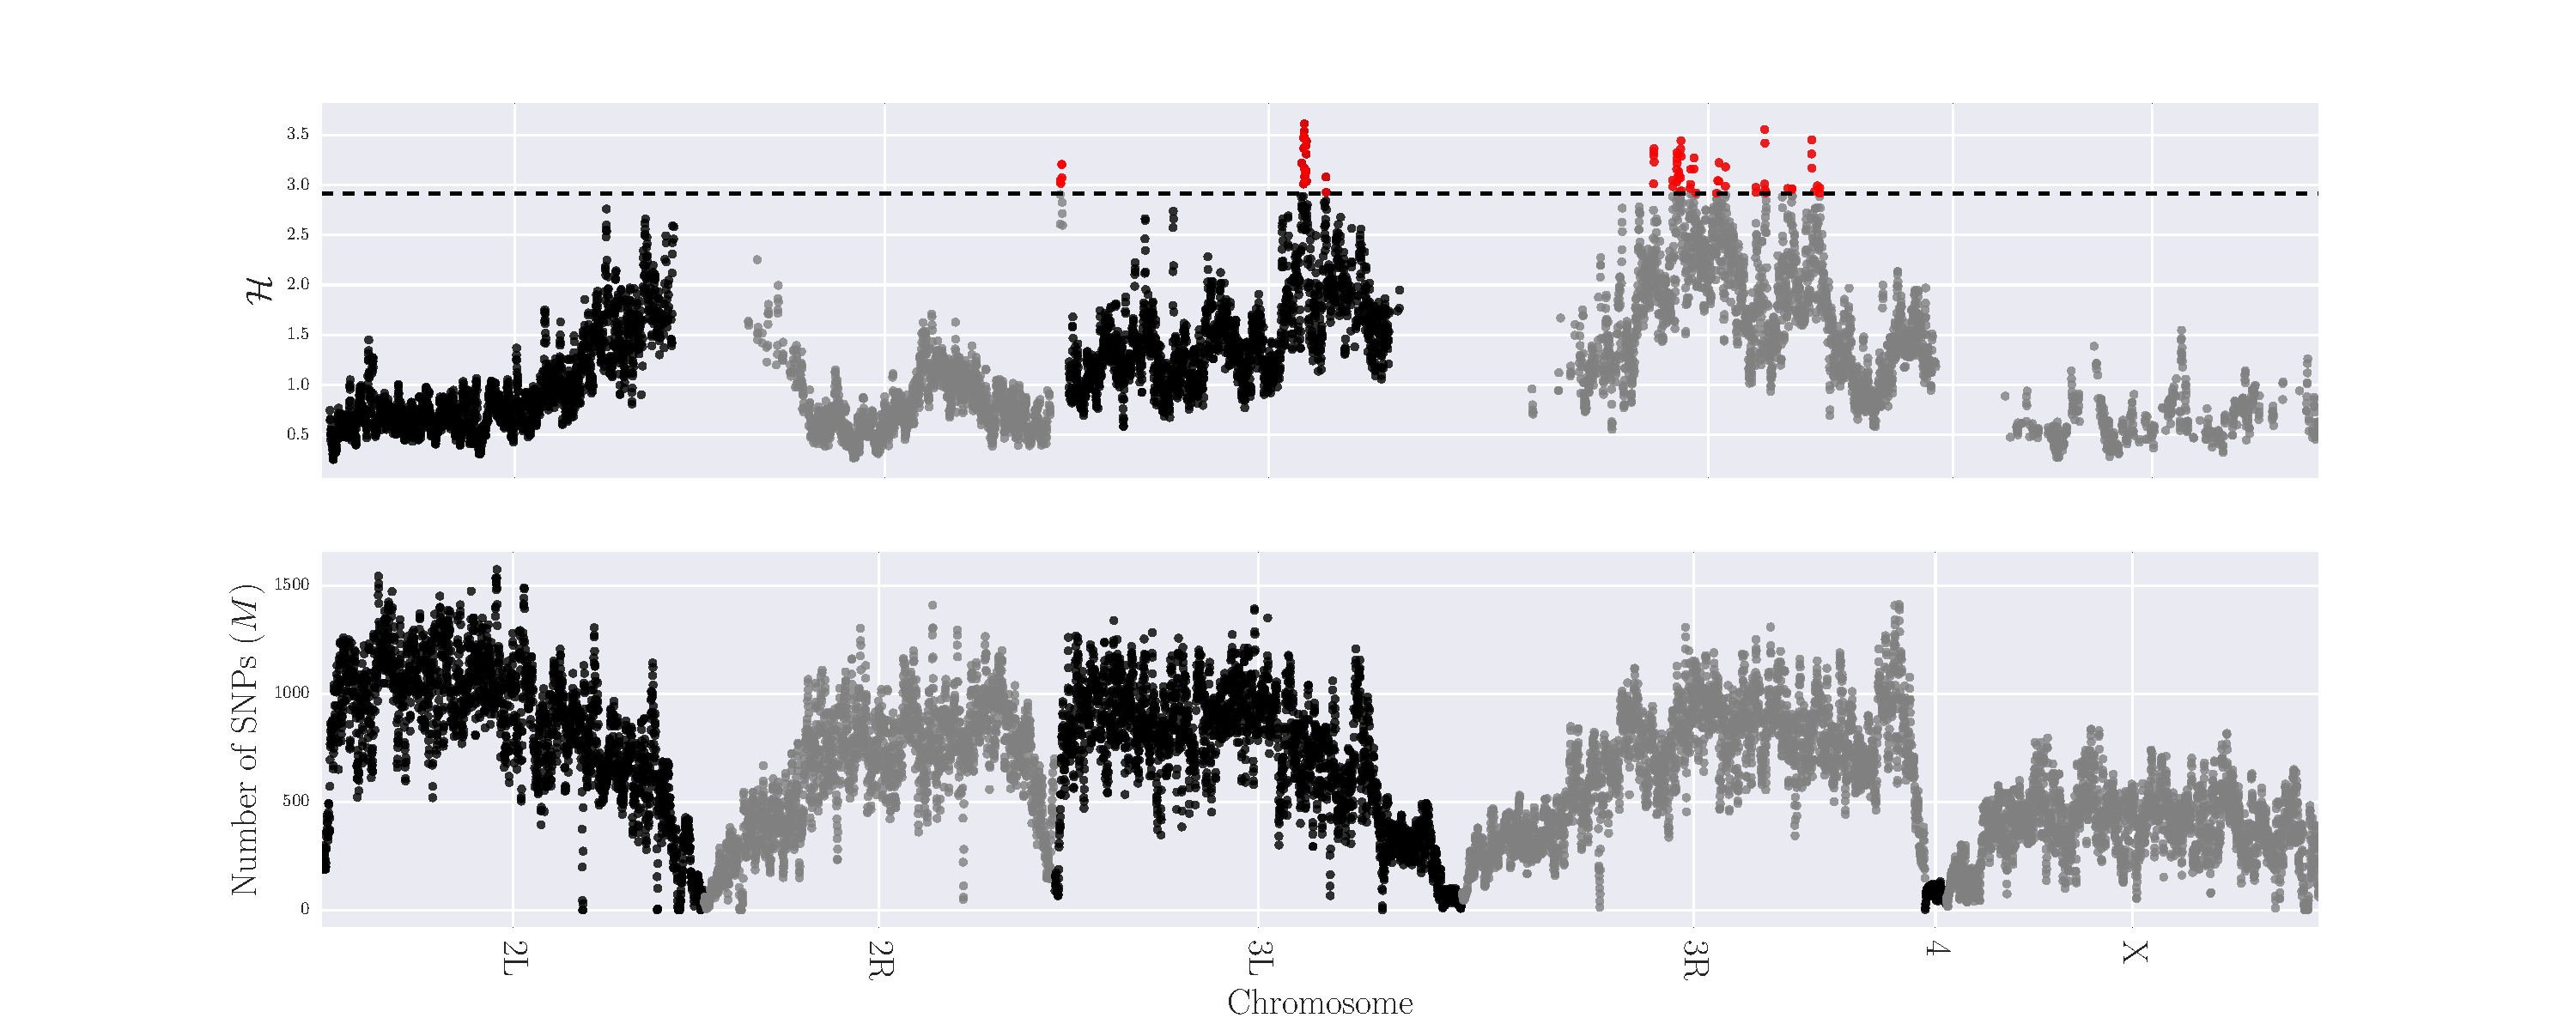
\includegraphics[width=\textwidth]{figures/manhattan.pdf}
	\caption{Manhattan plot of the composite $\Hc$ statistic (top) 
	and the number of SNPs (bottom) in 50Kbp sliding window with steps of 
	10Kbp. Regions in which their $\Hc$ statistic falls in top one percentile 
	distribution is denoted with red color. Pearson correlation between $M$ and 
	$\Hc$ of all windows is -0.03 and for the candidate regions is -0.27. This 
	nine-fold increase in correlation implies that the $\Hc$ statistic takes 
	more extreme values as the number of SNPs in the window is less than 
	expected ($\approx$1100).} 
	\label{fig:manhattan}
\end{figure}

\begin{figure}[H]
	\centering
	\includegraphics[width=\textwidth]{figures/{manhattan.min500snp}.pdf}
	\caption{Manhattan plot of the composite $\Hc$ statistic (top) 
		and the number of SNPs (bottom) in 50Kbp sliding window with steps of 
		10Kbp, excluding windows with less that 500 SNPs. Regions in which 
		their $\Hc$ statistic falls in top one percentile 
		distribution is denoted with red color. Pearson correlation between $M$ 
		and 
		$\Hc$ of all windows is -0.09 and for the candidate regions is -0.08. 
		This indicates the spurious effect of windows with low diversity is 
		removed from out study (potentially at cost of some false negatives). } 
	\label{fig:manhattancutoffed}
\end{figure}